\section{PianoRoll}\label{pianoRoll}

Accepts NoteProcessors: yes

Piano Roll - Notes

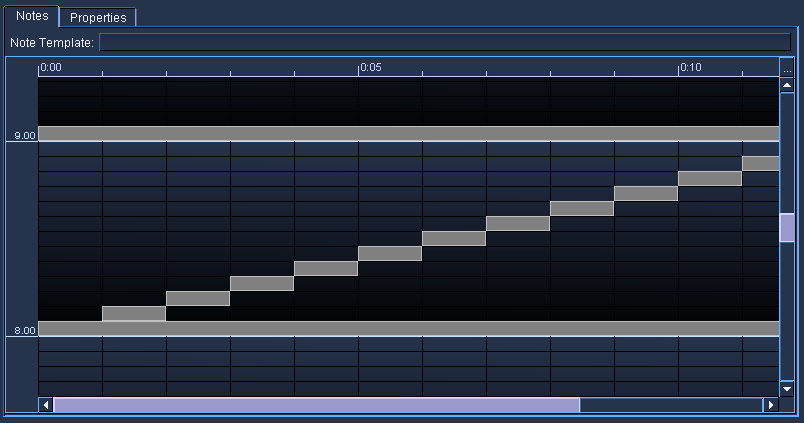
\includegraphics[width=1.00000\textwidth]{images/pianoRoll_notes.png}

The PianoRoll SoundObject is a graphical tool to enter in notes,
commonly available in many MIDI sequencer environments. This PianoRoll
is unique in that it is Microtonal: it supports loading any
\href{http://www.huygens-fokker.org/scala/}{Scala} scale file and
editing of notes adapts to that scale. For example, in the picture
above, the scale loaded is a Bohlen-Pierce scale with 13 tones to the
tritave. The PianoRoll above has adapted to that scale to show 13 scale
degrees per octave of its editor. The generated notes can output values
as either frequency or PCH notation (octave.scaleDegree). But don't
worry, if you're not interested in alternate tunings, the PianoRoll is
set by default to use 12-TET tuning, the "standard" tuning system in use
today.

The PianoRoll uses Note Template strings as a way to maintain
flexibility and be able to handle the open-ended nature of Csound's
instruments. Since the user who builds the instrument designs what each
pfield will mean(besides p1, p2, and p3), the Note Template string
should be made to match the instrument the user wants to use the
PianoRoll with. When the note is generated, certain special text values
(those enclosed in \textless{} and \textgreater{}) will be replaced by
values unique to the note.

For example, the following Note Template string:

\begin{verbatim}
      i<INSTR_ID> <START> <DUR> <FREQ> 0 1 1
    
\end{verbatim}

Will have the \textless{}INSTR\_ID\textgreater{} replaced with the value
set in the Piano Roll properties, \textless{}START\textgreater{}
replaced the start time for the note, \textless{}DUR\textgreater{}
replaced with the duration of the note, and
\textless{}FREQ\textgreater{} replaced with either a frequency or PCH
value, depending on how the Piano Roll is configured in its properties.
The other values will pass through as part of the note.

\begin{quote}
\textbf{Warning}

Caution should be used when creating a Note Template string to make sure
that there are enough spaces allowed between replacement strings. For
example, the following:

\begin{verbatim}
i<INSTR_ID> <START> <DUR> <FREQ> <FREQ> 0 1 1
      
\end{verbatim}

would result in:

\begin{verbatim}
i1 0 2 440 440 0 1 1
      
\end{verbatim}

while the following:

\begin{verbatim}
i<INSTR_ID> <START> <DUR> <FREQ><FREQ> 0 1 1
      
\end{verbatim}

which does not have proper space between the two
\textless{}FREQ\textgreater{} tags, results in:

\begin{verbatim}
i1 0 2 440440 0 1 1
      
\end{verbatim}
\end{quote}

The PianoRoll requires a bit of configuration before using. The
properties page below shows the properties that should be configure
before using the actual note drawing canvas.

Piano Roll - Notes - Properties

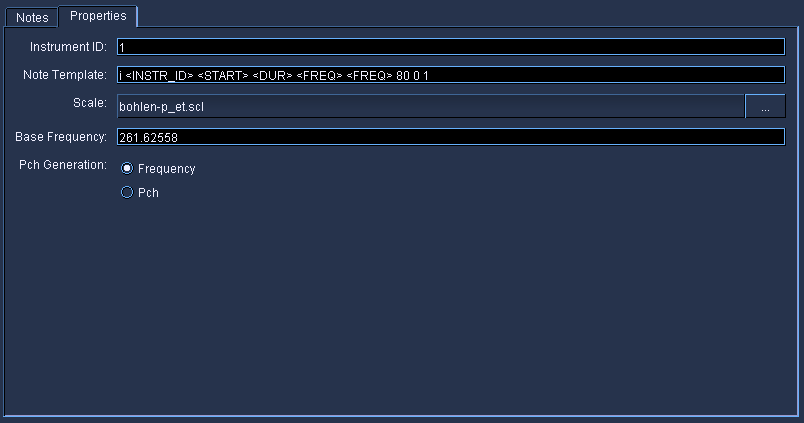
\includegraphics[width=1.00000\textwidth]{images/pianoRoll_properties.png}

\begin{description}
\item[Instrument ID]
Instrument name or number to be used when replacing
\textless{}INSTR\_ID\textgreater{} in Note template strings.
\item[Note Template]
The default note template when inserting notes. Notes make a copy of
this template string when created and edits to the note's string stay
with the note. Generally, you'll want to create a template string that
will match the instrument this PianoRoll will be used with.
\item[Scale]
The scale used with this PianoRoll. The PianoRoll defaults to a 12-TET
scale, the "standard" scale in use in Western classical and popular
music. Pressing the button labeled "..." will open a file browser for
selecting Scala scales to use in place of the default. After selecting a
scale, the PianoRoll will adjust the note canvas for the number of scale
degrees the newly selected scale contains.
\item[Base Frequency]
The base frequency of the scale for octave 8 and scale degree 0 (8.00).
Defaults to C below A440.
\item[Pch Generation]
Selects how the notes will generate their value to be used when
replacing the \textless{}FREQ\textgreater{} tag value in a note
template. The options are:

\begin{description}
\item[Frequency]
The value of the note's pitch expressed in terms of frequency in hertz.
This value is calculated using the chosen Scale for the PianoRoll.
\item[blue PCH]
Value of note expressed in blue PCH, a format similar to Csound PCH but
differs in that it does not allow fractional values. Values are
generated as "octave.scaleDegree" i.e. "8.22" would be octave 8 and
scale degree 22 in a scale that has 23 or more notes, or would wrap
around as it does in Csound PCH. If the scale had 12 scale degrees, the
"8.22" would be interpreted as "9.10". blue PCH is allowed as an option
to be used with blue PCH note processors and then to be used with the
Tuning NoteProcessor.
\item[MIDI]
When this Pch Generation method is chosen, a MIDI note value (0-127, 60
= Middle-C) is used for \textless{}FREQ\textgreater{} and the chosen
Scale will not be used. The display for the editor will automatically
switch to show octaves and notes for standard MIDI scale values. Using
MIDI note values is useful for instruments that exepct MIDI note values
such as the fluidsynth opcodes as well as midiout.
\end{description}
\end{description}

Piano Roll - Notes - Time Options

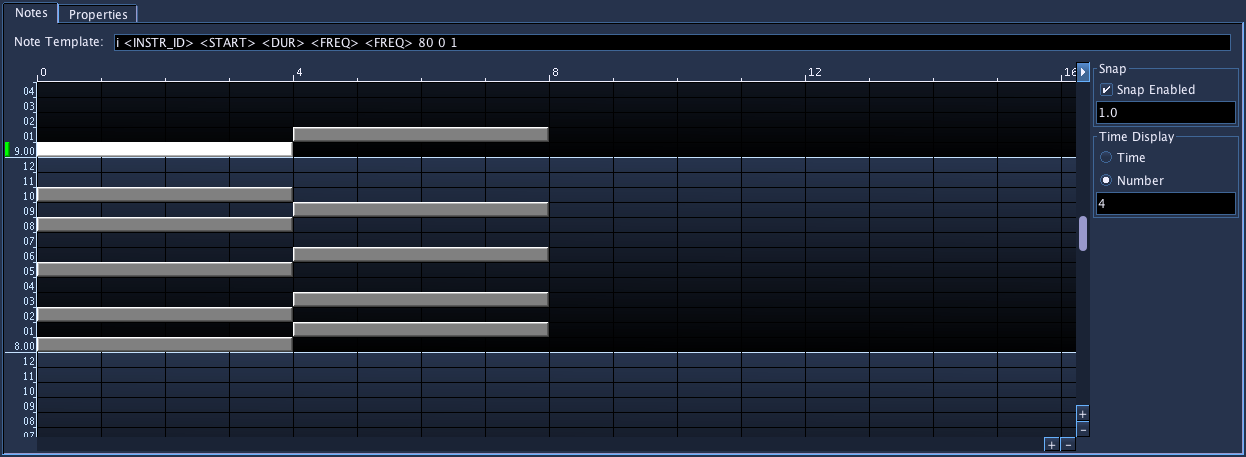
\includegraphics[width=1.00000\textwidth]{images/pianoRoll_notes_snap.png}

The Time Options in the PianoRoll are accessed and behave very much in
the same manner as those that are in the main timeline. The button
labelled "..." in the upper right corner of the PianoRoll canvas will
open and close the panel on the right that contains the properties.

\begin{description}
\item[Snap Enabled]
Enables snapping behavior on the timeline. If enabled, vertical lines
will be drawn at snap points, set by the value below it. In the
screenshot above, the snap is enabled and set to every 1.0 beats.
\item[Time Display]
Controls how the time in the time bar above the PianoRoll canvas will
display. The time value will show as time, while Number display will
display as integers. The number below show how often to put a label. In
the screenshot above, the Time Display is set to show a label in units
of time and at every 5.0 seconds.
\end{description}

To enter notes, hold down the shift key and press the left mouse button
down on the canvas. A note will be entered where you pressed and will be
set to resize as you move the mouse around. When you finally release the
mouse, the note will be finished entering.

After that, you can select notes by clicking on them or drag and
selecting notes by marquee. You can also press the shift key and click
on notes to add to the currently selected notes. You can then drag the
notes around by click a selected note and dragging. To resize a note,
select a single note, and after hilighted, move the mouse to the right
edge of the selected now, and then click and drag.

To remove a note or notes, select the notes, then press the del key.

To cut or copy a note, select a single note (only one note in the buffer
is currently supported), then press ctrl-x or ctrl-c to cut or copy,
respectively.

To paste, ctrl-click on the PianoNote canvas. (This is the same behavior
as pasting soundObjects on the main score timeline.)

To edit a note's template, select a single note. After selecting a note,
the text field for editing the note's template text will be enabled.
Here you can then edit the note's values.

\begin{quote}
\textbf{Note}

See the example .blue file in the blue/examples/soundObjects folder.
\end{quote}
